\chapter{Evaluation and Analysis}\label{chap:evaluation-and-analysis}


There are two types of target users in this platform. The first are the current ZeroZero's sports journalists who cover matches professionally, and have a platform where they do that already. They rely on it to update the match details on the ZeroZero platform. The second are casual people who like to follow lower division matches, due to the lack of coverage. With this in mind, different experiments were made, depending on the type of users and their use cases.

\section{Experiments Monitoring}

In order to better understand how the user is interacting with the application and pinpoint some aspects that might be worth improving, we intend to measure some aspects of the interaction. Next are some proposed metrics, which are relevant to this study. They are divided on their type for clearer understanding.

\begin{enumerate}
    \item Performance metrics:
    \begin{enumerate}
        \item Number of automatically-unsolved conflicts during an event per user
        \item Number of total generated conflicts
    \end{enumerate}
    \item Self-Reported metrics, asked in the form of a Likert scale\footnote{A typical item in a Likert scale is a statement to which respondents rate
    their level of agreement. The statement may be positive (e.g.,\ “The terminology used in this interface is clear”) or negative (e.g., “I found the navigation options confusing”). Usually a five-point scale of agreement like the following is used: 1. Strongly disagree 2. Disagree 3. Neither agree nor disagree 4. Agree 5. Strongly agree}, when appropriate:
    \begin{enumerate}
        \item The tool allowed the user to narrate the game without issues
        \item The user considered the number of conflicts... (1 - low; 5 - high)
        \item The user believed the events to correspond to the match's truth 
        \item The conflicts were easily to locate
        \item The conflicts were easy to solve \\
        \item The user has used another mean of communication with friends while following the match in order to discuss it (*) 
        \item The user would use the tool again in the future (*) \\
        \item Open answer to allow users to give whatever feedback they might have
    \end{enumerate}
\end{enumerate}

(*) Yes or No questions

\section{The Journalist Use-Case}
% often works alone, relies on the correct api sync (uses a more broad set of events)
% constant feddback-deployment loop
When covering a match, journalists usually work alone, as they are assigned different matches to cover. As such, they rarely face conflicts, but they also rely on the API syncronization feature heavily, as it is literally their job to keep the events they are covering up to date on the ZeroZero platform. This means they are an excelent feedback source on how the application works, overall. They provide the software verification feedback, but also validation.

Over the course of about five weeks, as soon as there was a usable product, they used it in production, pin-pointing issues and suggestions on how to make it better for their use-cases. There was a constant \say{deploy, feedback, adapt} loop, which allowed for a faster discovery of problems and their solutions. As of today, the ZeroZero Live platform as been used to cover more than 7 Euro2020 matches in production.

In those coverages, most of the times the events' count surpassed the 100th mark. However, as mentioned earlier, not many conflicts happened, since there was only one user per game.
When asked about the number of conflicts, journalists classified the number as very low, as expected. They, also as expected, believed the events corresponded to the match's truth. Finally, they were able to cover the matches without problems and would use the tool again, according to the questionnaires.

This validates the product on the journalist use-case. The tool allows CRUD\footnote{CRUD stands for Create-Read-Update-Delete, the four basic data-related operations a system can provide} operations and synchronizes to and from the ZeroZero's API, allowing them to insert, edit and delete events regarding a live match, which can be followed both on ZeroZero and on ZeroZero Live.

Next, the casual user's experience was evaluated, the analysis as available in the next subsection.

\section{The Casual User Use-Case}
% work in groups, crowdsourcing, in theory more conflicts
% portugal france experiment

Casual users have a slightly different use-case. While they too rely on CRUD operations in order to insert, edit and delete events, it's expected that they don't rely as much on ZeroZero API synchronization, as they will follow the game directly on ZeroZero Live. Additionally, a bigger difference relies on the number of participants per match, which is expected to be higher, contributing to the crowdsourcing nature of the tool. This raises the probability of event conflicts happening, which adds relevance to this work, regarding the automatic conflict resoliution. In this section, the system will be evaluated in that regard.

In order to prepare this type of experiments, a clone of ZeroZero Live was used. This clone was different in terms of features in order to focus on the conflict resolution. It also had no connection to the ZeroZero API, in terms of inserting events or making any changes to the teams for example. Additionally, authentication was not required which allowed for and experiment on a live relevant match, with no side effects on the ZeroZero platform. The chosen match was Portugal vs. France on the 23rd of June, regarding the Euro2020 group stage. Being a game involving Portugal's team, a long time rival as France, and the last match of the group stage, which Portugal could fail to pass, it was very important and many people would watch it, which meant many people to cover it and experiment the tool.

A total of 12 participants were included in the experiment. They were divided into 3 groups, which consisted of a control group (C1) and two experimental groups (E1 and E2). The control group had no automatic conflict resolution in place, whereas the other two groups had the automatic conflict resolution feature active. The application recorded the following metrics in order to help the analysis:

\begin{description}
    \item[Conflicts] Every time a conflict occurred, it was stored as a metric entry. When it was resolved, the entry was updated in order to know the conflict resolution time;
    \item[Number of Events] The total number of events in a match, as perceived by each user;
    \item[Number of Participants] The number of participants in a match (not necessarily participating actively)
\end{description}

In order to record these metrics, a new microservice was developed to record them. It exposed a simple HTTP API and reused the same existing MongoDB instance used for the reputation system, creating a new collection to store the metrics, for easy inspection.

\begin{table}[h]
    \centering
    \caption{Relation between number of events, participants and generated conflicts}
    \begin{tabular}{|l|l|l|l|}
        \hline
        \textbf{Metric}        & \textbf{C1} & \textbf{E1} & \textbf{E2} \\ \hline
        Number of Events       & 35 & 39 & 36 \\ \hline
        Number of Participants & 4  & 5  & 3  \\ \hline
        Number of Conflicts\footnotemark    & 3  & 1  & 0  \\ \hline
    \end{tabular}
    \label{table:num-events-participants-conflicts}
\end{table}

\footnotetext{The conflict on E1 was actually automatically resolved by the application.}

Table~\ref{table:num-events-participants-conflicts} shows the relation between the number of events, participants and generated conflicts. It is possible to see that the number of events does not vary much among the experiments. This can be explained by the fact that all participants were inexperienced in using the application, and watching the same match. For comparison purposes, the journalist that was covering the same match officially produced a total of 149 events, more than 3.8 times the most commented match (E1). We can also verify that the number of events does not scale with the number of participants, since E1 had two more participants than E2 (67\% increase), but only an 8.3\% increase in the number of events.

One can also note that the number of conflicts is higher on the environment where there was no automatic conflict resolution, as expected. However is not as high as expected --- only 8.6\% of the events conflicted. This can be explained by two factors: first, all users were watching the game remotelly, i.e., on the television or through some video stream on the internet. These transmissions are subject to variable delays, when compared to the game happening in real time, which resulted in different users watching the game out of sync compared to each other. Additionally, although no user had any prior experience with the application, different users have different times to insert events. All of this results in some users inputting events slower than others, and if someone inputs the same event earlier --- which would result in a conflict --- they end up stopping their input and avoiding the conflict altogether. Another phenonmenon that happened, still due to the reasons outlined above, was that the slower users would input the events after someone did, and inadvertedly overwrite them, since they had already received them at the moment of insertion, bypassing the conflicts.

\begin{table}[h]
    \centering
    \caption{Conflict resolution times and user perception}
    \begin{tabular}{|l|l|l|l|}
        \hline
        \textbf{Metric}                        & \textbf{C1} & \textbf{E1} & \textbf{E2} \\ \hline
        Number of Conflicts                    & 3  & 1  & 0  \\ \hline
        Average conflict resolution time (s)   & 92.7  & 0.7  & 0  \\ \hline
        Average percepted level of conflicts (1-5)     & 2  & 1.25  & 1  \\ \hline
    \end{tabular}
    \label{table:num-conflicts-time-perception}
\end{table}

\begin{figure}[h]
    \centering
    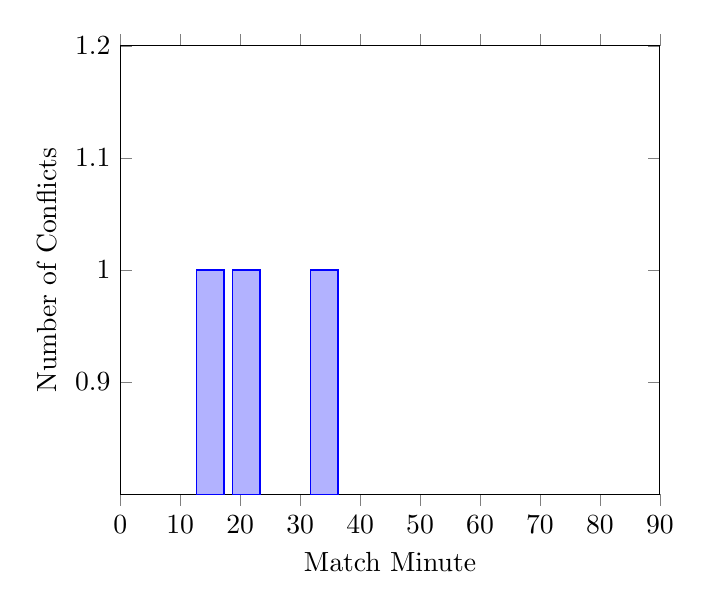
\begin{tikzpicture}
        \begin{axis} [ybar,xmin=0,xmax=90,xtick distance=10,
            ylabel=Number of Conflicts,
            xlabel=Match Minute
            ]
            \addplot coordinates {
                (15,1) 
                (21,1) 
                (34,1) 
            };
    \end{axis}
    
    \end{tikzpicture}
    \caption{Conflicts over game time (C1)}
    \label{chart:conflicts-over-time}
\end{figure}

As it can be seen from the data on Table~\ref{table:num-conflicts-time-perception}, in experiment C1 --- the control, where no automated conflict resolution was present --- there were 3 reported conflicts, which took, on average, 92.7 seconds to resolve. As expected, according to the questionnaire, the users perceived a higher amount of conflicts, although they still reported the level of conflicts to be only 2 points out of 5. On the other experiments, this value is lower --- 1 being the minimum --- which makes sense considering the amount of conflicts.

On figure~\ref{chart:conflicts-over-time}, one can notice that all of the conflicts happened on the first half, and most of them before the 30th minute. This confirms the idea that users are more active at the beginning of the match, especially considering that this match had many important events on the second half, including two goals, penalties and substitutions, which didn't lead to conflicts.


todo resolution time over time, satisfaçao com plat, would use again? localizar e resolver conflicts
